\subsection{UC4 - Interazione con lo staff}\label{usecase:4}
%diagramma dei casi d'uso 4
\begin{figure}[H]
  \centering
  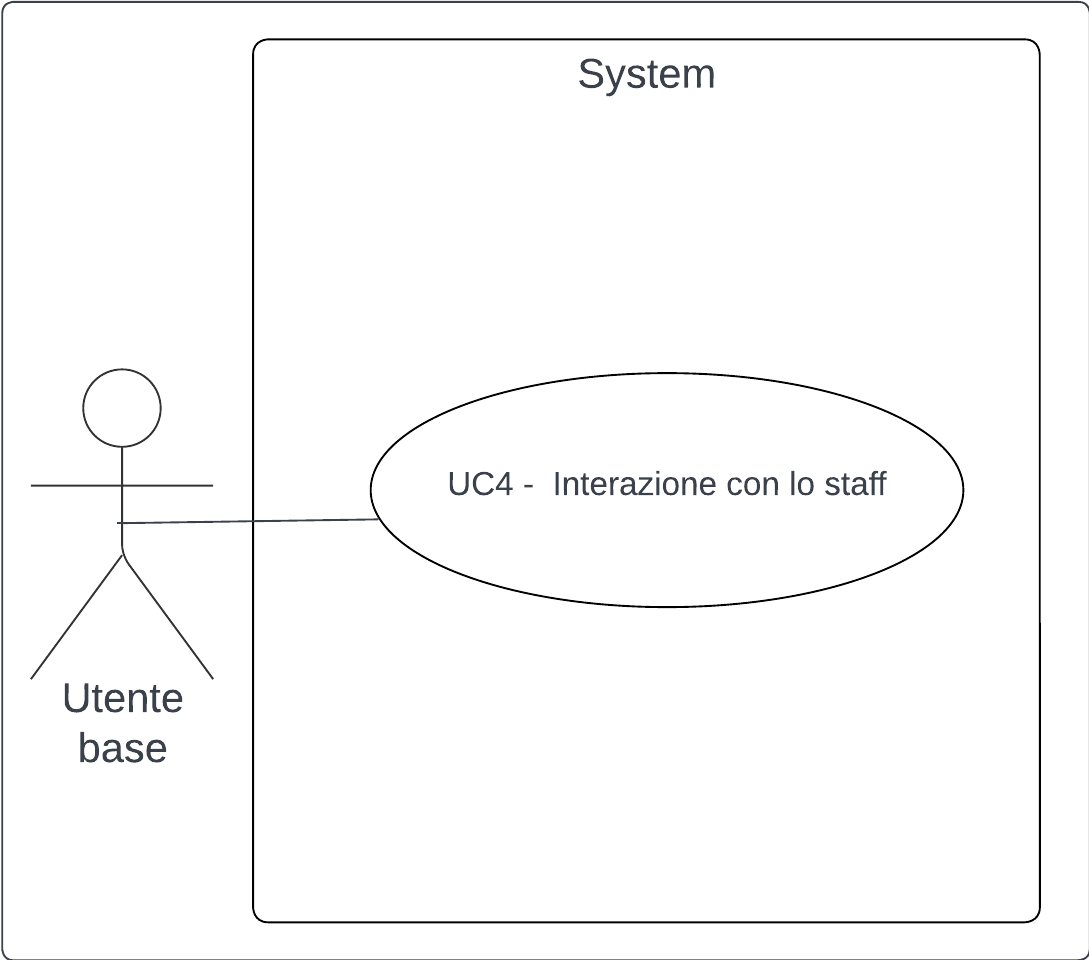
\includegraphics[width=0.7\textwidth]{ucd/UCD4.png}
\end{figure}
\textbf{Attori}:
\begin{itemize}
    \item Utente base
\end{itemize}
\textbf{Precondizioni}:
\begin{itemize}
    \item L'utente è autenticato dal sistema
\end{itemize}
\textbf{Postcondizioni}:
\begin{itemize}
    \item L'utente ha comunicato con l'amministratore del ristorante
\end{itemize}
\textbf{Scenari principali}:
\begin{enumerate}
    \item L'utente ricerca un ristorante (\nameref{usecase:24})
    \item L'utente seleziona un ristorante con cui comunicare
    \item L'utente può comunicare con l'amministratore e viceversa (\nameref{usecase:4_1})
    \item Durante la comunicazione verranno scambiati messaggi tramite notifica (\textit{push-notification}) (\nameref{usecase:4_2}) 
\end{enumerate}